% --- Template for thesis / report with tktltiki2 class ---
% 
% last updated 2013/02/15 for tkltiki2 v1.02

\documentclass[finnish]{tktltiki2}

% tktltiki2 automatically loads babel, so you can simply
% give the language parameter (e.g. finnish, swedish, english, british) as
% a parameter for the class: \documentclass[finnish]{tktltiki2}.
% The information on title and abstract is generated automatically depending on
% the language, see below if you need to change any of these manually.
% 
% Class options:
% - grading                 -- Print labels for grading information on the front page.
% - disablelastpagecounter  -- Disables the automatic generation of page number information
%                              in the abstract. See also \numberofpagesinformation{} command below.
%
% The class also respects the following options of article class:
%   10pt, 11pt, 12pt, final, draft, oneside, twoside,
%   openright, openany, onecolumn, twocolumn, leqno, fleqn
%
% The default font size is 11pt. The paper size used is A4, other sizes are not supported.
%
% rubber: module pdftex

% --- General packages ---

\usepackage[utf8]{inputenc}
\usepackage[T1]{fontenc}
\usepackage{lmodern}
\usepackage{microtype}
\usepackage{amsfonts,amsmath,amssymb,amsthm,booktabs,color,enumitem,graphicx}
\usepackage[pdftex,hidelinks]{hyperref}
\usepackage[ruled,vlined,linesnumbered]{algorithm2e}
\usepackage{caption}
\usepackage{float}
\usepackage{subcaption}

% Algorithm2e environment with "Algoritmi"-caption.
\newenvironment{finalgo}[1][htb]{
  \renewcommand{\algorithmcfname}{Algoritmi}
  \begin{algorithm}[#1]
}{\end{algorithm}}

% To be able to not numbering individual lines:
\let\oldnl\nl% Store \nl in \oldnl
\newcommand{\nonl}{\renewcommand{\nl}{\let\nl\oldnl}}

% Automatically set the PDF metadata fields
\makeatletter
\AtBeginDocument{\hypersetup{pdftitle = {\@title}, pdfauthor = {\@author}}}
\makeatother

% --- Language-related settings ---
%
% these should be modified according to your language

% babelbib for non-english bibliography using bibtex
\usepackage[fixlanguage]{babelbib}
\selectbiblanguage{finnish}

% add bibliography to the table of contents
\usepackage[nottoc]{tocbibind}
% tocbibind renames the bibliography, use the following to change it back
\settocbibname{Lähteet}

% --- Theorem environment definitions ---

\newtheorem{lau}{Lause}
\newtheorem{lem}[lau]{Lemma}
\newtheorem{kor}[lau]{Korollaari}

\theoremstyle{definition}
\newtheorem{maar}[lau]{Määritelmä}
\newtheorem{ong}{Ongelma}
\newtheorem{alg}[lau]{Algoritmi}
\newtheorem{esim}[lau]{Esimerkki}

\theoremstyle{remark}
\newtheorem*{huom}{Huomautus}

\DeclareMathOperator*{\argmin}{arg\, min}

% --- tktltiki2 options ---
%
% The following commands define the information used to generate title and
% abstract pages. The following entries should be always specified:

\title{Polunhakualgoritmit ja -järjestelmät}
\author{Rodion Efremov}
\date{\today}
\level{Kandidaatintutkielma-aine}
\abstract{Tiivistelmä.}

% The following can be used to specify keywords and classification of the paper:

\keywords{a, bb, ccc}

% classification according to ACM Computing Classification System (http://www.acm.org/about/class/)
% This is probably mostly relevant for computer scientists
% uncomment the following; contents of \classification will be printed under the abstract with a title
% "ACM Computing Classification System (CCS):"
% \classification{}

% If the automatic page number counting is not working as desired in your case,
% uncomment the following to manually set the number of pages displayed in the abstract page:
%
% \numberofpagesinformation{16 sivua + 10 sivua liitteissä}
%
% If you are not a computer scientist, you will want to uncomment the following by hand and specify
% your department, faculty and subject by hand:
%
% \faculty{Matemaattis-luonnontieteellinen}
% \department{Tietojenkäsittelytieteen laitos}
% \subject{Tietojenkäsittelytiede}
%
% If you are not from the University of Helsinki, then you will most likely want to set these also:
%
% \university{Helsingin Yliopisto}
% \universitylong{HELSINGIN YLIOPISTO --- HELSINGFORS UNIVERSITET --- UNIVERSITY OF HELSINKI} % displayed on the top of the abstract page
% \city{Helsinki}
%


\begin{document}

% --- Front matter ---

\frontmatter      % roman page numbering for front matter

\maketitle        % title page
\makeabstract     % abstract page

\tableofcontents  % table of contents

% --- Main matter ---

\mainmatter       % clear page, start arabic page numbering

\section{Johdanto}
Polunhaku painotetuissa tai painottamattomissa verkoissa on perustavanlaatuinen ongelma, joka ei ole mielenkiintoinen vain itsessään, vaan on toisinaan tarvittava alioperaatio muissa algoritmeissa. Esimerkiksi Edmond-Karpin algoritmi käyttää leveyssuuntaisen haun ratkaistaessaan maksimivuo-ongelmaa; multiple sequence alignment -ongelmaa on ruvettu viime vuosikymmeninä ratkomaan myös heuristisin polunhakualgoritmein.

Verkoista puhuttaessa verkko $G$ on kaksikko $(V, A)$, jossa $V$ on solmujen joukko, ja $A \subset V \times V$ on (suunnattujen) kaarien joukko. Suuntaamaton verkko $G' = (V, E)$ voidaan aina simuloida suunnatulla verkolla $G= (V, A)$ siten, että jokaista suuntaamatonta kaarta $\{ u, v \} \in E$ kohti laitetaan $A$:han kaaret $(u, v)$ ja $(v, u)$. (Suunnattu verkko on suuntamattoman yleistys.) Polunhakua varten, verkosta erotellaan kaksi solmua: lähtösolmu $s$ ja maalisolmu $t$. Jatkossa, $n = |V|$ ja $m = |E|$; näin esimerkiksi leveyssuuntaisen haun aikavaativuus on $O(n + m)$. Polku on $\gamma_k = \langle u_0, u_1, \dots, u_k \rangle$, missä mikään solmu ei esiinny yhtä kertaa enempää, ja verkossa on kaari $(u_i, u_{i + 1})$ jokaisella $i = 0, 1, \dots, k - 1$. Polkuun liittyvä kustannus on sen kaarien painojen summa, ja mitä tulee itse painoihin, ne oletetaan olevan ei-negatiivisia. Ei-painotettujen verkojen kohdalla, jokaisen kaaren paino oletetaan olevan 1.

% --- References ---
%
% bibtex is used to generate the bibliography. The babplain style
% will generate numeric references (e.g. [1]) appropriate for theoretical
% computer science. If you need alphanumeric references (e.g [Tur90]), use
%
% \bibliographystyle{babalpha-lf}
%
% instead.
\section{Tavallisimmat algoritmit}
Edsger W. Dijkstra esitti vuonna 1959 kuuluisan polunhakualgoritminsa, joka käy polynomisessa ajassa \cite{Dijkstra59}. Algoritmi voidaan pitää yhdistävän ''ahneuden'' (engl. \textit{greedy algorithm}), dynaamisen ohjelmoinnin ja inkrementaalisen lähestymistavan. Saatuaan lähtösolmun $s$, algoritmi laskee lyhimpien polkujen puun lähtien solmusta $s$ kunnes $t$ joutuu \textit{avoimeen listaan} (engl. \textit{open list; search frontier}), ja sitä kautta \textit{suljettuun listaan} (engl. \textit{closed list; settled node list}), jolloin lyhin $s, t$-polku on löytynyt. Hart et al. esittivät vuonna 1968 kuuluisan $A\ast$-algoritminsa,  joka -- samoin kuten Djikstran algoritmi -- ylläpitää mm. kunkin saavutetun solmun $u$ $g$-arvon $g(u)$, joka on toistaiseksi pienin kustannus lähtösolmusta $s$ solmuun $u$, ja joka on taattu olemaan pienin mahdollinen heti kun $u$ poistuu avoimesta listasta \cite{Hart68}. Erona on kuitenkin se, että $A\ast$ käyttää kunkin solmun $u$ prioriteettinä sen $f$-arvo, joka on siis $f(u) = g(u) + h(u)$, missö $h(u)$ on solmun $u$ optimistinen (eli aliarvioitu) etäisyys maalisolmuun. Intuitio tämän järjestelyn takana on se, että $A\ast$ ''tietää'' mihin suuntaan haku on suunnattava, jota pääsisi maalisolmuun, ainakin paremmin kuin Dijkstran algoritmi, jonka hakuavaruus kasvaa laajenevan pallon tavoin ''kaikkiin suuntiin''.
\begin{finalgo}
\nonl Monikkosijoitus \\
$\text{OPEN}, \text{CLOSED}, g, \pi = (\{ s \}, \emptyset, \{  (s, 0) \}, \{ (s, \textbf{nil}) \})$ \\
\While{$|\text{OPEN}| > 0$}{
 $u = \underset{x \in \text{OPEN}}{\argmin}\, g(x)$ \\
 \If{$x \textbf{\emph{ is }} t$}{
   \KwRet \textsc{Traceback-Path$(t, \pi, \textbf{nil})$}\\
 }
 $\text{OPEN} = \text{OPEN} - \{ u \}$ \\
 $\text{CLOSED} = \text{CLOSED} \cup \{ x \}$ \\
 \nonl Jokaisella solmun $x$ lapsisolmulla $u$, tee... \\
 \For{$(x, u) \in G.A$}{
   \If{$u \in \text{\upshape CLOSED}$}{
     $\textbf{continue}$ \\
   }
   $g' = g(x) + w(x, u)$ \\
   \If{$u \not \in \text{\upshape OPEN}$}{
     $\text{OPEN} = \text{OPEN} \cup \{ u \}$ \\
     $g(u) = g'$ \\
     $\pi(u) = x$ \\
   }
   \ElseIf{$g(u) > g'$}{
     $g(u) = g'$ \\
     $\pi(u) = x$ \\
   }
 }
}
\nonl Ei $s, t$ -polkua verkossa $G$. \\
\KwRet $\langle \rangle$ \\
\caption{\textsc{Dijkstra-Shortest-Path}$(G, s, t, w)$}
\label{alg:unidijkstra}
\label{Dijkstra}
\end{finalgo}
\noindent $A\ast$:n pseudokoodi on tasan sama kuin Dijkstran algoritmin (Algoritmi \ref{alg:unidijkstra}), paitsi että rivillä 3 $g(x)$:n sijasta on $f(x)$, jolle siis $f(x) = g(x) + h(x)$. Molemmat kutsuvat \textsc{Traceback-Path}-rutiinin, joka siis muodostaa lyhimmän polun ''edeltäjäpuusta'' (engl. \textit{predecessor tree}) ajassa $\Theta(N)$, missä $N$ on lyhimmän polun solmujen määrä. On huomattava, että $A\ast$ palautuu Dijkstran algoritmiin määrittelemällä $h(u) = 0$ jokaisella $u \in V$.
\begin{finalgo}
$u = x$ \\
$p = \langle  \rangle$ \\
\While{$u \textbf{\emph{ is not nil}}$}{
lisää $u$ $p$:n alkuun \\
$u = \pi(u)$
}
\nonl Kaksisuuntainen haku? \\
\If{$\pi_{REV} \textbf{\emph{ is not nil}}$}{
  $u = \pi_{REV}(x)$ \\
  \While{$u \textbf{\emph{ is not nil}}$}{
    lisää $u$ $p$:n loppuun \\
    $u = \pi_{REV}(u)$ \\
  }
}
\KwRet $p$ \\
\caption{\textsc{Traceback-Path}$(x, \pi, \pi_{REV})$}
\label{alg:tracebackpath}
\end{finalgo}

\section{Kaksisuuntainen haku}
Vaikka $A\ast$ on tyypillisesti tehokkaampi kuin Dijkstran algoritmi, käyttämällä \textit{kaksisuuntaista} hakua, voidaan päästää verrattavissa olevaan suorituskykyyn. Ajatus kaksisuuntaisuuden takana on se, että algoritmi kasvattaa kaksi hakupuuta, yksi normaaliin tapaan ja toinen maalisolmusta ihan kuin kaaret olisivat ''käännetty'' päinvastaiseen suuntaan, kunnes kaksi hakuavaruutta ''kohtaavat'' keskellä. Nyt jos lyhin polku koostuu $N$ kaaresta, ja verkon solmujen keskiarvoinen aste on $d$, tavallinen, eli yksisuuntainen haku tekee työn
\[
\sum_{i = 0}^N d^i,
\]
kun kaksisuuntainen olisi tehnyt vain
\[
2 \sum_{i = 0}^{\lceil N / 2 \rceil} d^i.
\]
Ylläoleva pätee leveyssuuntaiseen hakuun sellaisenaan, ja painotetun haun kohdalla voidaan saada yläraja kertomalla kunkin summan termin tekijällä $O(\log n)$. 

\subsection{Kaksisuuntainen Dijkstran algoritmi}
Ylläolevan analyysin nojalla, on selvä, että Dijkstran algoritmi hyötyy kaksisuuntaisuudesta, eikä edellytä minkäänlaista verkon esiprosessointia. Lisäksi, algoritmin vahvuutena suhteessa $A\ast$:iin ei ole pelkästään verrattavissa oleva tehokkuus, vaan myös heuristiikkafunktion tarpeettomuus. Alla $\mu$ on toistaiseksi lyhimmän polun kustannus, joka suorituksen alussa on $\infty$. Kun algoritmi löytää toistaiseksi lyhimmän polun hakuavaruuksien kohdatessa, ''välisolmu'' $m$ ja sen implikoiva kustannus $\mu$ päivitetään. Haku jatkuu siihen asti, kunnes molempien avointen listojen minimialkioiden kustannusten summa on vähintään $\mu$. 
\begin{finalgo}
$u = \underset{x \in \text{OPEN}}{\argmin} \, g(x)$ \\
\text{OPEN}  = \text{OPEN} - $\{ u \} $ \\
\text{CLOSED} = \text{CLOSED} $\cup \, \{ u \}$ \\
\For{$x \in e(u)$}{
  \If{$x \in \text{CLOSED}$}{
    \textbf{continue} \\
  }
  $g' = g(u)$ \\
  \If{$e(u) \textbf{\emph{ gives child nodes of }} u$}{
    \nonl ''Normaali'' haku.\\
    $g' = g' + w(u, x)$ \\
  }
  \Else{
  \nonl Käännetty haku.\\
  	$g' = g' + w(x, u)$ \\
  }
  \If{$x \not \in \text{OPEN}$}{
    $\text{OPEN} = \text{OPEN} \cup \{ x \} $ \\
    $g(x) = g'$ \\
    $\pi(x) = u$ \\
    \textsc{Update}$(x, \text{CLOSED}_2, g', g_2, \mu, m)$ \\
  }
  \ElseIf{$g(x) > g'$}{
    $g(x) = g'$ \\
    $\pi(x) = u$ \\
    \textsc{Update}$(x, \text{CLOSED}_2, g', g_2, \mu, m)$ \\
  }
}
\caption{\textsc{Expand}$(\text{OPEN, CLOSED, CLOSED}_2, g, g_2, \pi, \mu, m, e, w)$}
\label{alg:expand}
\end{finalgo}
\begin{finalgo}
\If{$x \in \text{CLOSED}$}{
   $p = g' + g(x)$ \\
   \If{$\mu > p$}{
     $\mu = p$ \\
     $m = x$ \\
   }
}
\caption{\textsc{Update}$(x, \text{CLOSED}, g', g, \mu, m)$}
\label{alg:update}
\end{finalgo}
Rutiini \textsc{Update} tarkistaa, että yhden hakusuunnan solmu on toisen suljetussa listassa, ja jos asia on niin, yrittää päivittää välisolmun.
\begin{finalgo}
$\text{OPEN}, \text{CLOSED}, g, \pi = \{ s \}, \emptyset, \{ (s, 0) \}, \{ (s, \textbf{nil}) \}$ \\
$\text{OPEN}_{REV}, \text{CLOSED}_{REV}, g_{REV}, \pi_{REV} = \{ t \}, \emptyset, \{ (t, 0) \}, \{ (t, \textbf{nil}) \}$ \\
$\mu = \infty$ \\
$m = \textbf{nil}$ \\ 
\While{$|\text{OPEN}| \cdot |\text{OPEN}_{REV}| > 0$}{
  \If{$m$ \textbf{\emph{is not nil}}}{
    $p = \textsc{Terminate}(\text{OPEN}, \text{OPEN}_{REV},$ \\
    $\phantom{p = \textsc{Terminate}(} g, g_{REV},$ \\
    $\phantom{p = \textsc{Terminate}(} \pi, \pi_{REV},$  \\
    $\phantom{p = \textsc{Terminate}(} \mu, m)$ \\
    \If{$p$ \textbf{\emph{is not nil}}}{
    	\KwRet $p$
    }
  }
  \nonl Triviaali kuormantasaus \\
  \If{$|\text{OPEN}| < |\text{OPEN}_{REV}|$}{
	$\textsc{Expand}(\text{OPEN},$ \\
	$\phantom{\textsc{Expand}(}\text{CLOSED},$ \\
	$\phantom{\textsc{Expand}(}\textsc{CLOSED}_{REV},$ \\ 
	$\phantom{\textsc{Expand}(}g, g_{REV}, \pi, \mu, m, e_f, w)$ \\
  }
  \Else{
	$\textsc{Expand}(\text{OPEN}_{REV},$ \\
	$\phantom{\textsc{Expand}(}\text{CLOSED}_{REV},$ \\
	$\phantom{\textsc{Expand}(}\textsc{CLOSED},$ \\ 
	$\phantom{\textsc{Expand}(}g_{REV}, g, \pi_{REV}, \mu, m, e_b, w)$ \\
  }
}
\KwRet $\langle  \rangle$ \\
\caption{\textsc{Bidirectional-Dijkstra-Shortest-Path}$(G, s, t, w)$}
\label{alg:bidijkstra}
\end{finalgo}
$e_f$ on kuvaus, jolle $e_f(u) = \{ v \in V \colon (u, v) \in A \}$ jokaisella $u \in V$, ja $e_b(u) = \{ v \in V \colon (v, u) \in A \}$. Molemmat siis määrittelevät ''laajentumisoperaattorit'' (engl. \textit{expansion operator}): $e_f$ normaalissa haussa, ja $e_b$ käännetyssä haussa.
\begin{finalgo}
\If{$\underset{x \in \text{OPEN}}{\min} g(x) + \underset{x \in \text{OPEN}_{REV}}{\min} g_{REV}(x) \geq \mu$}{
  \KwRet \textsc{Traceback-Path}$(m, \pi, \pi_{REV})$\\
}
\KwRet $\textbf{nil}$ \\
\caption{\textsc{Terminate}$(\text{OPEN}, \text{OPEN}_{REV}, g, g_{REV}, \pi, \pi_{REV}, \mu, m)$}
\label{alg:bidijkstraterminate}
\end{finalgo}

\subsection{Kaksisuuntainen $A\ast$}
Kaksisuuntaisen $A\ast$:n saa aikaan muuttamalla algoritmin \ref{alg:expand} rivillä 1 esiintyvä $g(x)$ $f(x)$:ksi ja muuttamalla \textsc{Terminate}-rutiinin ehto seuraavanlaiseksi:
\[
\max( \underset{x \in \textsc{OPEN}}{f(x)}, \underset{x \in \textsc{OPEN}_{REV}}{f_{REV}(x)} ) \geq \mu,
\]
jonka ehdotti Ira Pohl vuonna 1971 algoritmissaan BHPA \cite{Pohl71}.

Vuonna 2007 Taeg-Keun Whangbo ehdotti toisenlaisen kaksisuuntaisen heuristisen hakualgoritmin \cite{Whangbo07}. $h$-arvon sijasta, määritellään
\begin{align*}
l(x) &= \frac{(s - p) \cdot (x - p)}{ | s - p | }, x \in \text{OPEN}, \\
l_{REV}(x) &= \frac{(t - p) \cdot (x - p)}{ | t - p | }, x \in \text{OPEN}_{REV}.
\end{align*}
Kun kaksi hakuavaruutta kohtaavat solmussa $p$, piirretään $p$:n kautta kulkeva viiva $\Lambda$, joka on normaali sen viivan kanssa, joka kukee solmujen $s, t$ kautta. Nyt esimerkiksi jokaisella $x \in \text{OPEN}_{REV}$, $l_{REV}(x)$ on solmun $x$ etäisyys $\Lambda$:sta, ja uusi pysähtymisehto on
\begin{align*}
L^1_{\min} & \leq \underset{x \in \text{OPEN}}{\min} (g(x) + l(x)), \\
L^2_{\min} & \leq \underset{x \in \text{OPEN}_{REV}}{\min} (g_{REV}(x) + l_{REV}(x)),
\end{align*}
missä $L_{\min}^1$ on lyhimmän $s, p$ -polun kustannus normaalin haun puussa, ja $L_{\min}^2$ analogisesti lyhimmän $p, t$ -polun kustannus vastakkainsuuntaisessa haussa. Whangbo raportoi tavallisen $A\ast$:n vievän yhteensä 372 aikayksikköä laskettuna yhteen yli joukon hakuja. Samalla datalla BHPA vie 509 aikayksikköä, ja Whangbon variantti 209 aikayksikköä (huomaa BHPA:n vievän enemmän aikaa kuin tavallinen $A\ast$).

\section{Prioriteettijonon valinta}
Polkua hakiessa painotetussa verkossa joudutaan käyttäämään prioriteettijonoja, jotka ovat tarpeellisia pitääkseen haut optimaaleina, ja joiden oletetaan tarjoavan ainakin neljä operaatiota:
\begin{enumerate}
\item \textsc{Insert}$(H, x, k)$ tallettaakseen solmun $x$ sen prioriteetin $k$ kera,
\item \textsc{Decrease-Key}$(H, x, k)$ päivittääkseen solmun $x$ talletetun prioriteetin (pienemmäksi),
\item \textsc{Extract-Minimum}$(H)$ poistaakseen pienimmän prioriteetin omaava solmu, ja
\item \textsc{Is-Empty}$(H)$ varmistaakseen, että jonossa on vielä alkioita.
\end{enumerate}
Helpoin prioriteettijonorakenne (jatkossa vain ''keko''), jonka operaatiot (1) - (3) käyvät logaritmisessa ajassa, on binäärikeko. Tällaisella keolla Dijkstran ja $A\ast$-algoritmit käyvät kumpikin ajassa $O((m + n) \log n)$. Teoriassa edelläoleva ylläraja voidaan parantaa käyttämällä Fibonacci-kekoa, jonka lisäysoperaatio (1) käy eksaktissa vakioajassa, päivitysoperaatio (2) tasoitetussa vakioajassa, ja poisto-operaatio (3) tasoitetussa ajassa $O(\log n)$, jolloin haut voidaan suorittaa ajassa $O(m + n \log n)$. Huomaa, että kaikki tähän asti mainitut keot perustuvat vertailuihin, ja teoriassa enintään yksi operaatiosta \textsc{Insert} tai \textsc{Extract-Minimum} voi käydä eksaktissa tai tasoitetussa vakioajassa, ja toisen on käyttävä ajassa $\Omega(\log n)$, koska muuten algoritmi \ref{alg:genheapsort} tällaisella keolla rikkoisi vertailuihin perustuvan lajittelemisen informaatioteoreettisen rajan, joka on $\Omega(n \log n)$.
\begin{finalgo}
\nonl \text{Tyhjennä keko} \\
$H = \varnothing$ \\
\For{i = 1 \emph{\KwTo} |S|}{
  \nonl $S[i]$ on itsensä prioriteetti. \\
  \textsc{Insert}$(H, S[i], S[i])$ \\
}
\For{i = 1 \emph{\KwTo} |S|}{
  $S[i] = $\textsc{Extract-Minimum}$(H)$  \\
}
\caption{\textsc{Generic-Heap-Sort}($S, H$)}
\label{alg:genheapsort}
\end{finalgo}
Jos kuitenkin kaarien painot ovat kokonaislukuja, $O(m + n \log n)$-rajaa voidaan parantaa:
Mikkel Thorup esitti vuonna 2003 keon, jonka poisto-operaatio käy ajassa $O(\log \log \min n)$ ja muut operaatiot vakioajassa \cite{Thorup03}. Jos kuitenkin kokonaislukupainot ovat väliltä $[0, N)$, poisto-operaatio voidaan suorittaa ajassa $O(\log \log \min \{ n, N \})$. Nyt selvästi haun aikavaativuus tällaisella keolla on $O(m + n \log \log \min \{n, N \})$.

\section{Kaikkien parien lyhimmät polut}
Toisinaan on annettu $n$ solmua ja halutaan löytää lyhimmät polut kaikkien kahden eri solmun välillä. Yksi tehokkaimmista algoritmeista on Floyd-Warshallin algoritmi, joka käy ajassa $\Theta(n^3)$, eikä sen toiminta riipu kaarien määrästä $m$. Ellei kohdeverkko ole täysi ($m = o(n^2)$), Johnsonin algoritmi saattaa olla parempi valinta, sillä Fibonacci-keolla edellämainittu käy ajassa $O(n^2 \log n + nm)$. Ajatus Johnsonin algoritmissa on ensin tarkistaa, ettei verkossa ole negatiivisen kustannuksen omaava sykli, minkä jälkeen algoritmi ajaa $n$ kertaa Dijkstran algoritmin jokaisesta solmusta, ja jokaisella kerralla hakee kokonaisen lyhimpien polkujen puun. 

Ylläesitetyistä aikavaativuuksista ilmenee, ettei asianomaiset algoritmit ole tarpeeksi tehokkaita jo $n$:n arvoilla yli 10000. Jos kuitenkin ongelman koko sallii kaikkien parien algoritmin ajon, algoritmi palauttaa ''edeltäjämatriisin'' (engl. \textit{predecessor matrix}), josta $N$:n solmun lyhin polku voidaan rakentaa ajassa $\Theta(N)$, mitä ei pysty parantamaan tuon enempää, ei ainakaan ilman edistynempää algoritmiikkaa. (Ja vaikka voisikin, polun tulostaminen ja/tai piirtäminen on jo vähintään $\Omega(N)$.)

\section{Ruudukkoverkko ja jump point -haku}
Ruudukkoverkko (engl. \textit{grid graph}) on suuntamattoman verkon erikoistapaus, ja sen rakenne voidaan määritellä siten, että kullakin solmulla on kahden kokonaisluvun koordinaatti, eli solmujoukko on $\{ (x, y) \colon 1 \leq x \leq w, 1 \leq y \leq h \}$, missä $w$ on ruudukkoverkon leveys ja $h$ on sen korkeus. Nyt kun on annettu kaksi solmua $(x_1, y_1)$ ja $(x_2, y_2)$, jos vain yksi koordinaateista eroavat yksikön verran, kyseessä on vaaka- tai pystysuuntainen kaari ja sen painoksi asetetaan 1. Toisaalta, kun molemmat koordinaatit eroavat yksikön verran, kyseessä on vino kaari, jonka painoksi asetetaan $\sqrt{2}$. On selvää, että jo leveyssuuntainen haku on optimaali tällaisella verkolla, sillä aina kun se etenee vinottain, esim. solmusta $(x, y)$ solmuun $(x + 1, y - 1)$, se ohittaa kahden kaaren siirron solmun $(x + 1, y)$ tai $(x, y - 1)$ kautta, joka pidentäisi lyhimmän polun pituuden kahdella yksiköllä $\sqrt{2}$ sijaan. Heuristinen haku on kannattavaa tällaisella verkkotyypillä, sillä heuristiset funktiot kuten eukliidinen (tai Manhattan-metriikka, jos ei sallita vinot kaaret) on helppoa toteuttaa ilman esiprosessointia. Toisaalta, juuri tällaisella verkkotyypillä $A\ast$ kärsii polkujen ''symmetriasta'', kuten kuvasta \ref{fig:astarpathsymmetry} ilmenee. Jos siis solmujen $s$ ja $t$ molemmat koordinaatit eroavat, $A\ast$ kasvattaa suunnikkaanmuotoisen hakuavaruuden solmusta $s$ solmuun $t$, sillä niiden välissä on monta saman kustannuksen omaavaa polkua. Kuten yleensä erikoistapauksiin rajoittuessa, polunhaku ruudukolla voidaan tehdä paljon tehokkaammin. Vuonna 2011 Harabor ja Grastien esittivät ''jump point search'' -nimisen $A\ast$:n muunnelman, joka karsii pois polkusymmetriat ja etenee ''hyppien'' yli monen solmun siinä, missä muut algoritmit etenevät jokaisen välisolmun kautta \cite{Harabor11}.
\begin{figure}
  \centering
  \begin{subfigure}[h]{0.45\textwidth}
    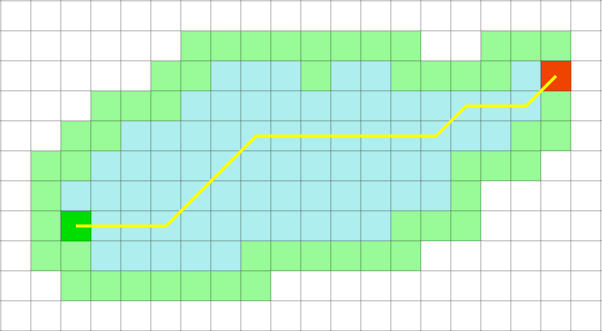
\includegraphics[clip=true,trim = 8px 8px 8px 8px,width=\textwidth,keepaspectratio]{AStarSearch}
    \caption{$A\ast$-haku}
    \label{fig:astarpathsymmetry}
  \end{subfigure}
  ~
  \begin{subfigure}[h]{0.45\textwidth}
    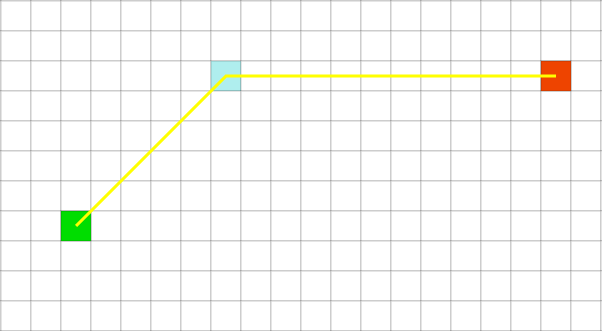
\includegraphics[clip=true,trim = 8px 8px 8px 8px,width=\textwidth,keepaspectratio]{JumpPointSearch}
    \caption{Jump point -haku}
  \end{subfigure}
  \caption{Polkusymmetria}
\end{figure}

\section{Dijkstran algoritmi kaarivipuilla}
Vuonna 2007 Möhring et al. esittivät mielenkiintoisen tavan nopeuttaa Dijkstran algoritmi \cite{Mohring07}. Ajatuksena on osittaa suunnatun verkon $G=(V, A)$ solmujoukko osioihin $V_1, \dots, V_p$ siten, että
\[
\bigcup_{i = 1}^p V_i = V,
\]
ja $V_i \cap V_j = \emptyset$ jokaisella $i \neq j$. Ositus voidaan toteuttaa kuvauksella $r \colon V \to \{1, \dots, p\}$. Kustakin osiosta $V_i$ puhuttaessa, sen ''rajasolmut'' (engl. \textit{boundary nodes}) määritellään joukkona
\[
B_i = \{ v \in V_i \colon \exists(u, v) \in A \text{ siten että } r(v) \neq r(u) \}.
\]
Lisäksi, järjestelmä liittää jokaiseen verkon kaareen ''kaarivipuvektorin'' (engl. \textit{arc-flag vector}), jota voidaan toteuttaa $p$:n bitin bittivektorina. Nyt jokaisella osiolla $V_i$ järjestelmän esiprosessointialgoritmi ajaa ''takaperin'' tavallisen Dijkstran algoritmi kustakin rajasolmusta $b \in B_i$, ja asettaa tuloksena syntyvässä lyhimpien polkujen puussa jokaisen kaaren $a$ kohdalla $a$:n vipuvektorin $r(b)$:s bitti päälle. Tuloksena syntyvässä järjestelmässä, hakiessa polkua solmuun $t$, nopeutettu Dijkstran algoritmi voi karsia kaikki ne kaaret, joiden vektorin $r(t)$:s bitti ei ole päällä, ainakin niin kauan kunnes haku pääsee samaan osioon solmun $t$ kanssa. Tekniikka voidaan siis nähdä tasopainoilevan tavallisen Dijkstran algoritmin ($V_1 = V$) ja kaikkien parien algoritmin (kukin solmu on osio) välillä.

\subsection{Ositustekniikat}
 Kuten ylläolevasta kävi ilmi, ''kaarivipu''-Dijkstra vaatii verkon solmujen osituksen, minkä jälkeen joudutaan esiprosessoimaan koko verkko. Koska esiprosessoinnin aika riipuu lineaarisesti kaikkien osioiden kaikkien rajasolmujen yhteenlasketusta määrästä, jälkimmäisen minimointi on toivottavaa. 
 
 Mikäli on annettu kunkin solmun koordinaatit tasossa, helpoin tapa osioida verkko (''ruudukointi'') on jakaa pienin, kaikki solmut sisältävä suorakulmio $w$ sarakkeeseen ja $h$ riviin. Tämä ei kuitenkaan ole vailla ongelmia: esimerkiksi viidenkymmenen neliökilometrin osio pääkaupunkiseudulla sisältäisi paljon enemmän infrastruktuuria kuin jokin samankokoinen alue Kainuun maakunnassa. Asia voidaan parantaa käyttämällä ''nelipuita'' (engl. \textit{quad-tree}): koko suorakulmio jaetaan neljään, samankokoiseen suorakulmioon, minkä jälkeen jaetaan jälkimmäiset, ja niin edelleen pysäyttäen jaon niiden suorakulmioiden kohdalla, joissa on enintään $\kappa$ solmua ($\kappa$ annetaan nelipuualgoritmille parametrina). Tämä ottaa solmujakauman jo paremmin kuin ruudukointi, mutta ei niin hyvin kuin $kd$-puu (engl. \textit{$kd$-tree}), joka lajittelee kaikkien solmujen listan ensin esimerkiksi $x$-koordinaattien perusteella, poimii mediaanialkion $x$-koordinaatin $x_{mid}$, ja implisiittisesti jakaa koko listan kahteen osalistaan $V_{\leq}$ ja $V_{>}$, missä $V_{\ast} = \{ x \in V \colon x \ast x_{mid}\}$, minkä jälkeen lajitellaan $V_{\leq}$ ja $V_{>}$, mutta jo $y$-koordinaattien perusteella, ja jako pysähtyy niiden solmujoukkojen kohdalla, joissa on enintään $\kappa$ solmua (tässäkin $\kappa$ on nelipuulle annettu parametri).
 
 Neljäs tapa, jota Möhring et al. ovat tarkastelleet, on vuonna 1998 kehitetty METIS \cite{Karypis98}, joka ei edes tarvitse solmukoordinaatteja. Järjestelmä toimii siten, että syöteverkosta $G_i$ muodostetaan verkko $G_{i + 1}$ siten, että $G_i$:ssä korvataan ''tiheästi'' kytketyt solmut yhdellä solmulla verkossa $G_{i + 1}$, ja niin jatkaen pääsee tarpeeksi pieneen verkkoon $G_{min}$, jonka osittaminen on tarpeeksi tehokasta. Kun $G_{min}$ on ositettu, kuljetaan redusointiketjussa takaperin ja laajennetaan väliverkot $G_{min - 1}, \dots, G_1$, kunnes päästään alkuperäiseen verkkoon $G_0 = G$.
 
\subsection{Tulokset}
Koska kaksisuuntainen haku on mahdollista myös kaarivipujärjestelmässä, asia vaatii vain sen, että kuhunkin kaaren liitetään kaksi vipuvektoria, yksi kutakin hakusuuntaa varten. Tällaisella algoritmilla Möhring et al. raportoivat nopeutuksen suhteessa tavalliseen Dijkstran algoritmiin olleen yli 500 noin yhden miljoonan solmun ja $2.5 \times 10^6$ kaaren verkolla.
 
\section{Polunhaku ja Multiple Sequence Alignment \\-ongelma}

\section{Lyhimmät polut ja rinnakkaisuus}
Toistaiseksi lyhimpien polkujen haku ei juuri antanut paljon aihetta rinnakkaistamiseen. Vuonna 1998 Meyer ja Sanders esittivät $\Delta$-stepping -nimisen algoritminsa, joka asettaa kunkin saavutetun solmun $u$ omaan ''koriin'' (engl. \textit{bucket}) numero $i$ aina, kun $g(u) \in [(i - 1)\Delta, i\Delta)$, jolloin kukin säie käsittelee vain osan kaikista koreista. $2^{19}$ solmun verkolla, jonka keskiarvoinen asteen 3, Meyer ja Sanders raportoivat peräkkäisen (engl. \textit{sequential}) version olleen 3.1 kertaa nopeampi kuin ''optimoitu'' Dijkstran algoritmi, ja 16 suorittimen hajautetussa järjestelmässä nopeutus 9.2 on mitattu suhteessa peräkkäiseen $\Delta$-stepping -algoritmiin. On huomattava, että algoritminsa toiminta riippuu $\Delta$:n arvosta, ja Meyer et al. ehdottavat arvon $\Delta = 4/d$, missä $d$ on keskiarvoinen solmun aste.

Rinnakkaistamiseen liittyvien käytännön ongelmista huolimatta, myös kaksisuuntaisen $A\ast$:n variantti nimeltään NBA$\ast$ sai rinnakkaisen version: PNBA$\ast$ käyttää kaksi säiettä, kukin omaa hakusuuntaa varten, ja sisältää suhteellisen vähän synkronoinnin tarvetta \cite{Rios}. Esimerkiksi, 15-palapelillä (engl. \textit{15-puzzle}), NBA$\ast$ löysi lyhimmän 58 siirron polun noin 2.5 kertaa nopeammin kuin $A\ast$, ja PNBA$\ast$ oli noin tasan kaksi kertaa nopeampi kuin edellinen.

On huomattava, että rinnakkaistaessa algoritmeja, ei ole mahdollista saada mielivaltaisen suuria nopeutuksia jo Amdahlin lain nojalla, jonka mukaan maksimaalinen nopeutus on
\[
\frac{1}{(1 - P) + \frac{P}{N}},
\]
missä $N$ on suorittimien määrä ja $P \in (0, 1]$ on sen laskennan suhteellinen osuus, jota voidaan tehdä rinnakkain, eikä $P$ ole koskaan 0, sillä jokaisessa rinnakkaisessa laskennassa joudutaan luomaan säikeet, mikä on ainakin osittain peräkkäinen operaatio.

\bibliographystyle{babplain-lf}
\bibliography{refs}


% --- Appendices ---

% uncomment the following

% \newpage
% \appendix
% 
% \section{Esimerkkiliite}

\end{document}